\section{\LaTeX~Coding Best Practices} \label{sec:Conclusion}
This section outlines some key coding functions that are extremely helpful when working with \LaTeX.

\subsection{Internal Document Referencing}

\LaTeX\ automatically handles referencing using its built in \verb*|\ref{}| or the often preferred \textit{cleveref} userpackage \verb*|\cref{}|. 
How referencing works is a \verb*|\label{}| is placed at a section title (\verb*|\label{sec:}|), in an equation (\verb*|\label{eqn:}|), in a table (\verb*|\label{tab:}|), or in a figure (\verb*|\label{fig:}|). 
With a label in place, say in \cref{fig:mufasaB2}, the Cleveref is used to add a reference in text. For example, \cref{fig:mufasaB2} is labelled \textit{fig:mufasaB2}, so to reference it in-text the code is \verb*|\cref{fig:mufasaB2}|.

\subsection{Citations}

Always check the style and expected format of references for the journal/conference/university the paper will be submitted to. 
When citing, ensure the bibtex file has all the required information to be displayed according to the journal/conference/university requirements. 
An example bibtex entry for work by \citeauthor{BenThesis} \cite{BenThesis} is provided as follows: 

\begin{verbatim}
	@mastersthesis{BenThesis,
		author = {Durante, Benjamin Joseph},
		pages = {1--128},
		school = {University of Calgary]},
		title = {Flying and Handling Qualities of Small-Scale Supersonic Uncrewed Aerial Vehicles},
		note = {{Avaliable: \url{https://dx.doi.org/10.11575/PRISM/40789}}},
		type = {{[Master's} Thesis},
		year = {2023}
	}
\end{verbatim}

\noindent
Additional BibTex entry formats are found online, with common types being \verb*|@article{}|, \verb*|@inproceedings{}|, \verb*|@techreport{}|, \verb*|@phdthesis{}|, \verb*|@book{}|, and \verb*|@misc{}|. 
 
Based on the BibTex identification name (ex. \textit{BenThesis} above) references are easily cited in-text and added to the bibliography. Multiple commands are used to automatically cite a work depending on the presentation desired:
\begin{itemize}
	\item \verb*|\cite{BenThesis}| cites the text numerically as follows: \cite{BenThesis},
	\item \verb*|\citep{BenThesis}| acts very similarily to the previous command in IEEE and AIAA as follows: \citep{BenThesis}, however this command behaves differently with the APA citation style, 
	\item \verb*|\citeauthor{BenThesis}\cite{BenThesis}| automatically fills in the authors name and then adds the numerical reference, automatically linking both, as follows: \citeauthor {BenThesis} \cite{BenThesis}.
\end{itemize}


\subsection{Diagram Creation} \label{sec:diagramCreation}

Diagrams should appear crisp, ideally they are vector files meaning they can be infinitely zoomed in without getting blurry. 
Diagram text should align with the document text exactly. One way to ensure diagram text always matches the \LaTeX\ document text is by creating the diagrams in InkScape. 
The diagram creation video is outlined in the following YouTube video: \url{https://youtu.be/NbHKJNMsYqE?si=W-XXTR8T_Izss_j1}. 
Note, this YouTube example only works for InkScape Version~1.1 (\url{https://inkscape.org/release/inkscape-1.1/?latest=1%29}). 

\begin{figure}[hbt!]
	\centering
	\captionsetup{width=0.7\textwidth}
	%\includegraphics[width=0.7\textwidth]{Photos/MUFASA/MUFASA-ISO-Frames-BodyLength.png}
	\def\svgwidth{0.7\textwidth}
	\input{Photos/MUFASA/MUFASA-ISO-Frames-BodyLength.eps_tex}
	\caption{MUFASA B aerodynamic design and coordinate system.}
	\label{fig:mufasaB2}
	\hfill
\end{figure}

\noindent 
This type of figure is generated using the following commands: 

\begin{verbatim}
	\begin{figure}[hbt!]
		\centering
		\captionsetup{width=0.7\textwidth}
		%\includegraphics[width=0.7\textwidth]{Photos/MUFASA/MUFASA-ISO-Frames-BodyLength.png}
		\def\svgwidth{0.7\textwidth}
		\input{Photos/MUFASA/MUFASA-ISO-Frames-BodyLength.eps_tex}
		\caption{MUFASA B aerodynamic design and coordinate system.}
		\label{fig:mufasaB2}
		\hfill
	\end{figure}
\end{verbatim}

\subsection{Equations}
When coding an equation, carefully consider what is a variable and what is a label. 
Variables should be in math text, while labels should be in regular text. 
For example, in \cref{eqn:netForce}, $F_{\text{net}}$ is net force, not force as a function of variables $n \times e \times t$. 
Regular text can be inserted into an equation via the \verb*|\text{}| command. 

\begin{equation} \label{eqn:netForce}
	F_{\text{net}} = F_{\text{aero}} + F_{\text{g}} + F_{\text{T}}
\end{equation}


\subsection{Figure Creation}
\subsection{Custom Variable Creation}
\newcommand{\ap}{ArduPilot}
Local document variables are a way to aid in typing repetitive words or numerical values. 
These custom variables also aid in document consistency when referring to repeated words or values. 
An example of using locally defined document variables is creating a command to represent the word \textit{ArduPilot}. 
Due to the letters in \textit{ArduPilot}, it is an awkward word to type and a coding shorthand is created using the command: \verb*|\newcommand{\ap}{ArduPilot}|. 
Now, by typing \verb*|\ap\|, the word \ap\ is seamlessly inserted into the text. 
Note that the \verb*|\| following the \verb*|\ap| indicates a space should be left following the word \ap.

\LaTeX\ variables also work when inserted into InkScape generated figures, as outlined in the following YouTube video: \url{https://youtu.be/r0G44lxhTwc?si=SVSKCUj6mTy4rGCN}. 
Using variables in a diagram increases writing efficiency as it reduces the need to manually regenerate diagrams to change a variable when using the workflow presented in \Cref{sec:diagramCreation}. 